% Options for packages loaded elsewhere
\PassOptionsToPackage{unicode}{hyperref}
\PassOptionsToPackage{hyphens}{url}
\PassOptionsToPackage{dvipsnames,svgnames,x11names}{xcolor}
%
\documentclass[
  letterpaper,
  DIV=11,
  numbers=noendperiod]{scrartcl}

\usepackage{amsmath,amssymb}
\usepackage{iftex}
\ifPDFTeX
  \usepackage[T1]{fontenc}
  \usepackage[utf8]{inputenc}
  \usepackage{textcomp} % provide euro and other symbols
\else % if luatex or xetex
  \usepackage{unicode-math}
  \defaultfontfeatures{Scale=MatchLowercase}
  \defaultfontfeatures[\rmfamily]{Ligatures=TeX,Scale=1}
\fi
\usepackage{lmodern}
\ifPDFTeX\else  
    % xetex/luatex font selection
\fi
% Use upquote if available, for straight quotes in verbatim environments
\IfFileExists{upquote.sty}{\usepackage{upquote}}{}
\IfFileExists{microtype.sty}{% use microtype if available
  \usepackage[]{microtype}
  \UseMicrotypeSet[protrusion]{basicmath} % disable protrusion for tt fonts
}{}
\makeatletter
\@ifundefined{KOMAClassName}{% if non-KOMA class
  \IfFileExists{parskip.sty}{%
    \usepackage{parskip}
  }{% else
    \setlength{\parindent}{0pt}
    \setlength{\parskip}{6pt plus 2pt minus 1pt}}
}{% if KOMA class
  \KOMAoptions{parskip=half}}
\makeatother
\usepackage{xcolor}
\setlength{\emergencystretch}{3em} % prevent overfull lines
\setcounter{secnumdepth}{-\maxdimen} % remove section numbering
% Make \paragraph and \subparagraph free-standing
\ifx\paragraph\undefined\else
  \let\oldparagraph\paragraph
  \renewcommand{\paragraph}[1]{\oldparagraph{#1}\mbox{}}
\fi
\ifx\subparagraph\undefined\else
  \let\oldsubparagraph\subparagraph
  \renewcommand{\subparagraph}[1]{\oldsubparagraph{#1}\mbox{}}
\fi


\providecommand{\tightlist}{%
  \setlength{\itemsep}{0pt}\setlength{\parskip}{0pt}}\usepackage{longtable,booktabs,array}
\usepackage{calc} % for calculating minipage widths
% Correct order of tables after \paragraph or \subparagraph
\usepackage{etoolbox}
\makeatletter
\patchcmd\longtable{\par}{\if@noskipsec\mbox{}\fi\par}{}{}
\makeatother
% Allow footnotes in longtable head/foot
\IfFileExists{footnotehyper.sty}{\usepackage{footnotehyper}}{\usepackage{footnote}}
\makesavenoteenv{longtable}
\usepackage{graphicx}
\makeatletter
\def\maxwidth{\ifdim\Gin@nat@width>\linewidth\linewidth\else\Gin@nat@width\fi}
\def\maxheight{\ifdim\Gin@nat@height>\textheight\textheight\else\Gin@nat@height\fi}
\makeatother
% Scale images if necessary, so that they will not overflow the page
% margins by default, and it is still possible to overwrite the defaults
% using explicit options in \includegraphics[width, height, ...]{}
\setkeys{Gin}{width=\maxwidth,height=\maxheight,keepaspectratio}
% Set default figure placement to htbp
\makeatletter
\def\fps@figure{htbp}
\makeatother
% definitions for citeproc citations
\NewDocumentCommand\citeproctext{}{}
\NewDocumentCommand\citeproc{mm}{%
  \begingroup\def\citeproctext{#2}\cite{#1}\endgroup}
\makeatletter
 % allow citations to break across lines
 \let\@cite@ofmt\@firstofone
 % avoid brackets around text for \cite:
 \def\@biblabel#1{}
 \def\@cite#1#2{{#1\if@tempswa , #2\fi}}
\makeatother
\newlength{\cslhangindent}
\setlength{\cslhangindent}{1.5em}
\newlength{\csllabelwidth}
\setlength{\csllabelwidth}{3em}
\newenvironment{CSLReferences}[2] % #1 hanging-indent, #2 entry-spacing
 {\begin{list}{}{%
  \setlength{\itemindent}{0pt}
  \setlength{\leftmargin}{0pt}
  \setlength{\parsep}{0pt}
  % turn on hanging indent if param 1 is 1
  \ifodd #1
   \setlength{\leftmargin}{\cslhangindent}
   \setlength{\itemindent}{-1\cslhangindent}
  \fi
  % set entry spacing
  \setlength{\itemsep}{#2\baselineskip}}}
 {\end{list}}
\usepackage{calc}
\newcommand{\CSLBlock}[1]{\hfill\break\parbox[t]{\linewidth}{\strut\ignorespaces#1\strut}}
\newcommand{\CSLLeftMargin}[1]{\parbox[t]{\csllabelwidth}{\strut#1\strut}}
\newcommand{\CSLRightInline}[1]{\parbox[t]{\linewidth - \csllabelwidth}{\strut#1\strut}}
\newcommand{\CSLIndent}[1]{\hspace{\cslhangindent}#1}

\KOMAoption{captions}{tableheading}
\makeatletter
\@ifpackageloaded{caption}{}{\usepackage{caption}}
\AtBeginDocument{%
\ifdefined\contentsname
  \renewcommand*\contentsname{Table of contents}
\else
  \newcommand\contentsname{Table of contents}
\fi
\ifdefined\listfigurename
  \renewcommand*\listfigurename{List of Figures}
\else
  \newcommand\listfigurename{List of Figures}
\fi
\ifdefined\listtablename
  \renewcommand*\listtablename{List of Tables}
\else
  \newcommand\listtablename{List of Tables}
\fi
\ifdefined\figurename
  \renewcommand*\figurename{Figure}
\else
  \newcommand\figurename{Figure}
\fi
\ifdefined\tablename
  \renewcommand*\tablename{Table}
\else
  \newcommand\tablename{Table}
\fi
}
\@ifpackageloaded{float}{}{\usepackage{float}}
\floatstyle{ruled}
\@ifundefined{c@chapter}{\newfloat{codelisting}{h}{lop}}{\newfloat{codelisting}{h}{lop}[chapter]}
\floatname{codelisting}{Listing}
\newcommand*\listoflistings{\listof{codelisting}{List of Listings}}
\makeatother
\makeatletter
\makeatother
\makeatletter
\@ifpackageloaded{caption}{}{\usepackage{caption}}
\@ifpackageloaded{subcaption}{}{\usepackage{subcaption}}
\makeatother
\ifLuaTeX
  \usepackage{selnolig}  % disable illegal ligatures
\fi
\usepackage{bookmark}

\IfFileExists{xurl.sty}{\usepackage{xurl}}{} % add URL line breaks if available
\urlstyle{same} % disable monospaced font for URLs
\hypersetup{
  pdftitle={Bioeconomy Accounting: Methods and Pilot Application to 13 Latin American Economies},
  colorlinks=true,
  linkcolor={blue},
  filecolor={Maroon},
  citecolor={Blue},
  urlcolor={Blue},
  pdfcreator={LaTeX via pandoc}}

\title{Bioeconomy Accounting: Methods and Pilot Application to 13 Latin
American Economies}
\author{Renato Vargas \and Andrés Mondaini \and Adrián
Rodríguez \and Mónica Rodríguez \and Irene Alvarado \and Paul Wander}
\date{}

\begin{document}
\maketitle
\begin{abstract}
We propose a practical methodology to estimate Bioeconomic Satellite
Accounts following the rules outlined in the System of National Accounts
for analytical extensions. This methodology reaggregates classifications
within the Supply and Use tables of this system to highlight the
economic contribution of inputs and outputs driven by biological
resources for all economic activities. In contrast to similar studies,
we suggest that an \emph{a priori} classification of economic activities
as either ``bioeconomic'' or ``non-bioeconomic'' underestimates value
added by biological resources that fall outside the predetermined
activities. Instead, we assess the economic contribution driven by
biological resources for all economic activities and propose direct and
indirect methods to rank them according to their importance for
bioeconomic policy. We exemplify the methodology with the cases of
Guatemala and Costa Rica, and we provide estimates for 13 economies of
Latin America and The Caribbean.
\end{abstract}

\subsection{Introduction}\label{introduction}

In 2018, the Costa Rican Government published that country's National
Bioeconomy Strategy, following an internationally agreed definition
crafted in the context of the German Bioeconomy Council (German
Bioeconomy Council, 2018), which states that the Bioeconomy is:

\begin{quote}
``The production, use, conservation, and regeneration of biological
resources, including the knowledge, science, technology, and innovation
related to these resources, to provide information, products, processes,
and services to all economic sectors, with the goal of advancing toward
a sustainable economy (Gobierno de Costa Rica, 2020).''
\end{quote}

Additionally, this strategy defines ``biological resources'' within the
framework as \textbf{i)} biomass cultivated to produce food, fodder,
fibers, and energy; \textbf{ii)} biomass from marine resources and that
produced through aquaculture; \textbf{iii)} forest biomass, especially
that cultivated for use in the forestry and paper industries, as well as
that legally extracted from natural ecosystems; \textbf{iv)} residual
biomass from the agricultural, fishing and aquaculture, forestry, and
agro-industrial sectors; \textbf{v)} biomass that can be recovered from
urban waste; \textbf{vi)} liquid waste from livestock and human
activities; and \textbf{vii)} terrestrial and marine biodiversity,
including the biodiversity of inland waters.

Public policies informed by data have been shown to provide
opportunities to build upon what works and understand why it works
(Bowers \& Testa, 2019). While Costa Rica has a long tradition in the
production of environmental accounts (BCCR, 2021b) following the System
of Environmental and Economic Accounts---SEEA---(European Commission,
Economic Cooperation, Development, United Nations, \& World Bank, 2013),
their Environmental Accounts Council identified a gap in the assessment
of the direct and indirect contribution of biological resources to the
economy that officials needed to close to design better policies around
the subject.

Given the richness of information regarding biological resources that is
collected to assess the economic performance of the country, we were
granted the opportunity to close this gap by extending the System of
National Accounts (SNA), the framework with which Gross Domestic Product
(GDP) is measured, among many other indicators, to highlight the
contribution of those resources through Bioeconomy Sataellite Accounting
(BSA) for Costa Rica (Vargas, Alvarado, Rodríguez, Rodríguez, \& Wander,
2022). The SNA manual (European Commission et al., 2009, p. 523)
provides clear guidelines on how to develop analytical
extensions---specifically \emph{Key Sector Accounts} and \emph{Satellite
Accounts}---and we chose to adhere to those guidelines to avoid
deviations from SNA's concepts and accounting rules and mantain
comparability with traditional economic indicators. In particular, we
focused on reaggregating classifications of the Supply and Use Tables
(SUTs) that provide detail for what is known as the production account
within SNA.

This strict adherence to the principles of SNA and the standarization
procedure developed to handle SUT data in the case of Costa Rica,
allowed us to readily extend this exercise to 13 Latin American
economies. This was possible because these economies have made their
Supply and Use tables publicly available and this information has been
centralized in a repository (ECLAC, 2021). Relying on the SNA
principles, definitions, classifications, and accounting rules also gave
us an opportunity to express results related to the Bioeconomy using
concepts that are easily understood by policy-makers because of their
widespread use in economic performance communications and analysis.

\subsection{Data and Methods}\label{data-and-methods}

\subsubsection{Supply and Use Tables as data
sources}\label{supply-and-use-tables-as-data-sources}

The main source of information for BSAs are SUTs from SNA (European
Commission et al., 2009), which are multi-dimensional matrices that show
in great detail the production and import of goods and services by
economic activities in a country and how those are used, either in the
production process itself as inputs, by other agents in the economy, or
by the rest of the world. The different areas of these tables describe a
flow of transactions in the economy. All transactions (columns) show
detailed information for all products (rows) identified in a given
economy. The production transaction in the Supply Table and the
intermediate consumption transaction in the Use Table are further
disaggregated by economic activities (columns). The detail of products
is arranged according to national adaptations of the Central Product
Classification---CPC---(United Nations, 2015) and economic activities
are arranged according to the International Standard Industrial
Classification of All Economic Activities---ISIC---(United Nations,
2008).

In the case of the Supply Table, the sequence of those transactions
(columns) describes a flow where different products (rows) are produced
by economic activities at basic prices (i.e., the price at the farm
gate, factory, or commercial establishment). This output is then
combined with imports free of insurance and freight costs to form the
supply at basic prices. However, this is not the price paid by economic
agents. In its way to market, taxes on products are added to the basic
price supply, minus any subsidies received, followed by distribution
margins (transportation and trade costs). This results in the total
supply at purchaser's or market prices, found in the last column of the
table, which represents what is available for purchase by the same
economic agents in the use table. For these additional columns of
transactions, the product detail (rows) is mantained, but not the
economic activity detail.

The Use Table shows how the supply from the last column of the Supply
Table is purchased by economic agents for various purposes at market
prices, expressed in the form of different transactions. Similar to the
production above, this table shows Intermediate Consumption, which
refers to the purchase of inputs by economic activities used to produce
the goods and services in the first table (essentially, the production
recipe for each economic activity). The portion of the supply that does
not become an input in the production process remains available on the
market for other domestic and foreign economic agents. The other
transactions in the remaining columns illustrate that these goods and
services can be exported; consumed by households, nonprofit institutions
serving households (NPISH), and the general government; or they can be
used as durable goods in gross capital formation; moved in or out of
storage to be consumed in a different accounting period (changes in
inventories); or get sold as valuable items. It is important to note
that, row by row (product detail), the Total Use column equals the last
column of the Supply Table, adhering to the economic principle of
equality between supply and demand.

\subsubsection{Characterizing the Bioeconomy using product
classifications: a two step
procedure}\label{characterizing-the-bioeconomy-using-product-classifications-a-two-step-procedure}

Countries use adaptations of the international classifications of
economic activities and products to focus on those elements that are
important to their economic structure. In most cases, there is a
one-to-one correspondence between international classifications and
their national adaptations. However, this is not always the case,
because there might be key national activities and products unique to
the country that do not have an international counterpart. In other
cases, there could be a match at one level of disaggregation but not at
another, due to the way some categories are combined. This is reflected,
for example, in the vertical integration of certain industries where the
same economic activity produces a primary sector good while it also
provides services related to that production in a manner that's
indistinguishable in their financial statements, making it practically
impossible to separate them. This, for example, could result in a
product category comprising a mix of codes from an agricultural division
and a services division. For this reason, it is necessary to follow a
two-step procedure:

\begin{itemize}
\item
  In the first step, we compare the different products from the CPC
  classification against the internationally agreed definition of the
  Bioeconomy shown in the introductory paragraphs (German Bioeconomy
  Council, 2018), in general, and that of biological resources in
  particular (Gobierno de Costa Rica, 2020), and we decide whether the
  product matches any of its parts conceptually. It should be clarified
  that, at the highest levels of disaggregation, certain services, which
  may not initially appear to be directly related to the Bioeconomy,
  have been taken into consideration in this first step, based on the
  argument that they could not exist without the prior existence of a
  Bioeconomic product. For example, the category \emph{62123 Retail
  trade services of meat, poultry, and game in non-specialized stores}
  refers to a trade service, but its purpose and existence are so
  closely tied to bioeconomic products that it could not exist without
  the prior production of \emph{21111 Fresh or chilled beef} or
  \emph{21121 Fresh or chilled chicken} one step back in the supply
  chain, as well as \emph{02111 Cattle} and \emph{02151 Chickens} two
  steps back in the production chain. For this reason, these have been
  categorized as Characteristic of the Bioeconomy. This is also
  consistent with the Bioeconomy definition, which includes services.
  Nevertheless, national adaptations in the following step do not have
  this level of disaggregation and thus a binary approach, even with
  these caveats, is impossible and we resort to the creation of a
  partial category termed Extended Characteristic of the Bioeconomy.
  Resulting equivalence tables are included in the Supplementary
  Information (SI) section.
\item
  In a second step, we analyze each element of the national product
  classification and evaluate how each corresponding code aligns with
  the binary identification from the international classification of
  previous step. Often, national classifications bundle together product
  categories at a level that is sensible for field or record data
  collection. This results in three possible outcomes 1) 100\% of the
  products within the national category belong to the Bioeconomy,
  according to the international classification (Bioeconomy products);
  2) only some of the products within the national category belong to
  the Bioeconomy, according to the international classification (we call
  those Bioeconomy Extended products); and 3) none of the activities or
  products within the category belong to the Bioeconomy, according to
  the international classification (Non-Bioeconomy Products).
\end{itemize}

Once this rearrangement is completed, we describe the Bioeconomy using
traditional macroeconomic aggregates like output, intermediate
consumption, imports, exports, taxes on products, and gross capital
formation disaggregated for Bioeconomy products, Bioeconomy Extended
products, and Non-Bioeconomy products.

\subsubsection{Bioeconomic Value Added and GDP: a divergence from other
studies}\label{bioeconomic-value-added-and-gdp-a-divergence-from-other-studies}

The output of every economic activity less its intermediate consumption
(its inputs) leaves a remainder called Value Added, which is then
available for distribution among the owners of capital, laborers, and
the government. Value Added is similar in business accounting to the
concept of profits, which are what remains after deducting costs from
total sales. The only difference is that in National Accounts, payments
to employees are not deducted as costs. The sum of the individual Value
Added of all economic activities, plus taxes, less subsidies, equals
GDP. One important fact about Value Added is that it is calculated by
economic activity and not by product and this poses a challenge for the
Bioeconomy.

Initial efforts in the nascent gray literature classify economic
activities as Bioeconomic or Non-Bioeconomic \emph{a priori} based on
whether their primary production is a bioeconomic product or not, as
defined in the previous section. Then they add together, either all, or
a fraction of their Value Added (VA) as a proxy for the ``Bioeconomic
GDP''. We understand that this approach as a necessary compromise,
because ``biological resource'' is a quality of products, but VA and GDP
are aggregates that are estimated at the economic activity or total
economy level. While these first approximations have provided valuable
estimates of the size of the Bioeconomy, this \emph{a priori}
determination of bioeconomic activities has at least three important
limitations.

\begin{enumerate}
\def\labelenumi{\arabic{enumi}.}
\tightlist
\item
  Within SUTs economic activities can produce more than one product and,
  in turn, any product in the Economy can be produced by more than one
  activity. Bioeconomic products could be part of the secondary
  production of activities that have not been deemed as Bioeconomic.
  Since the value added of these activities is not included in the
  estimation of the Bioeconomy, this would lead to an under estimation
  of the contribution of bioeconomic products.
\item
  Secondary production of Non-Bioeconomic products within an activity
  classified as Bioeconomic \emph{a priori} could be a non-trivial share
  of its output. Taking that activity's entire Value Added as
  Bioeconomic would lead to an over estimation of the contribution of
  bioeconomic products to the total economy.
\item
  \emph{A priori} classification of economic activities as Bioeconomic
  is based on observed values at the time of compilation. There are
  activities in the present that might not have biological inputs or
  outputs, but which could have them in the future. For example, in a
  given country, there might be zero biological resources used in
  construction, rendering that activity as non-bioeconomic, but with the
  advent of biomaterials and other innovations, this could change in the
  future and housing could be constructed with ``live'' materials. Not
  belonging to the Bioeconomy at the time of first compilation, these
  future developments would be overlooked. Alternatively, reclassifying
  them as Bioeconomic o Bioeconomic Extended in the future would
  introduce inconsistencies to time series.
\end{enumerate}

Instead, we propose that the Bioeconomy within an economic activity is a
continuum. All economic activities might use, as part of their
production recipe between 0 and 100 percent of bioeconomic inputs for
the production of its output, which can itself be between 0 and 100
percent bioeconomic. We can then estimate the direct fraction of
economic value that is enabled by biological resources by adjusting
Value Added by any of these percentages. This leads to a more accurate
estimation of the Bioeconomy by minimizing the sources of under or over
estimation discussed above.

This is a criteria that we developed only after trying the first
approach and finding these pockets of under or over representation of
the Bioeconomy outside \emph{a priori} determined bioeconomic
activities. Our original estimates for Costa Rica (Vargas et al., 2022)
showed that the bioeconomy described with this first method was of about
12.0\% of Gross Value Added. Using our proposed approach allowed us to
correct our under and overvalued estimation of the Bioeconomy, which
resulted in a contribution of 15.7\% of Gross Value Added in the case of
an output based fraction estimation and 17.2\% in the case of an
intermediate consumption based fraction estimation.

\subsection{Results}\label{results}

This section presents a comparative series of results that highlight the
contribution of biological resources to 13 economies of Latin America
and the Caribbean, focusing on several macroeconomic aggregates. As an
example of the information generated for each country, we provide a
compact version of the Bioeconomy SUTs with data from Guatemala for the
year 2019---the most recent year available in ECLAC's repository (ECLAC,
2021)---and insights at economic sector level from the Costa Rican case.

\subsubsection{Bioeconomy SUT: The case of
Guatemala}\label{bioeconomy-sut-the-case-of-guatemala}

In the Supply Table (Table~\ref{tbl-gtm19-sup}), the most important
categories correspond to the output (OP) or the production of goods and
services, which are divided into bioeconomy, extended bioeconomy, and
non-bioeconomy. For presentation purposes, all 152 products and services
from the Guatemalan economy, as published in the ECLAC repository
(ECLAC, 2021), are aggregated into these three categories. In the case
of the use table (Table~\ref{tbl-gtm19-use}), the same three bioeconomic
aggregations are displayed, but this time they represent the
intermediate consumption and final consumption of the same 152 products
(row data). In other words, purchases of inputs by activities for
production (intermediate consumption); purchases of households,
nonprofit institutions, and the government as consumers; gross capital
formation (i.e.~the purchase of durable goods, valuable objects, and
changes in inventories); and exports.

\begin{table}

\caption{\label{tbl-gtm19-sup}Guatemala: Condensed Bioeconomy Supply
Table\\
(Million GTQ at current prices, 2019)}

\centering{

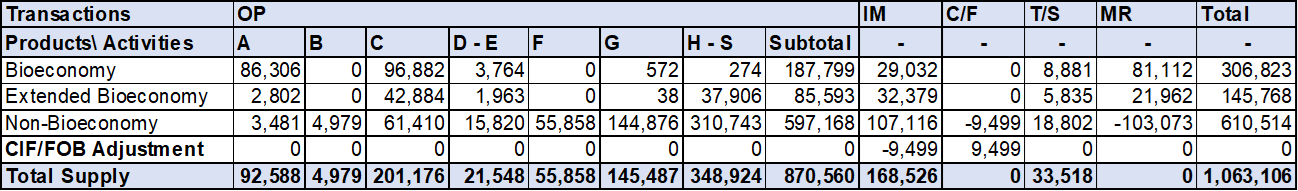
\includegraphics{images/clipboard-3904732418.png}

}

\end{table}%

Transactions: OP. Output; IM. Imports; C/F. CIF/FOB Adjustment; T/S.
Taxes less subsidies; MR. Trade and transport margins. Groups of
Activities: A. Agriculture; B. Mining; C. Manufacturing; D-E Other
Utilities \& Water; F. Construction; G. Wholesale and Retail Trade; H-S.
Other services.

The flow of information from left to right in Table~\ref{tbl-gtm19-sup}
shows output (OP) at producer prices (i.e., the price at the farm gate
or factory), to which we then add imports free of insurance and freight
costs to form the supply of goods and services in the economy at basic
prices. The transactions in the following columns add detail on
insurance and freight costs, taxes less subsidies on products, and
distribution margins (i.e., transportation and marketing costs), which
are added to bring these products to consumers. The last column shows,
row by row, the availability of each good and service in the economy at
market prices in the case of supply (Table~\ref{tbl-gtm19-sup}), which
is equal to total use (in Table~\ref{tbl-gtm19-use}) row by row.

Table~\ref{tbl-gtm19-sup} shows an output of 324.2 billion QTQ in
bioeconomic products, which corresponds to 28.7\% of the total supply at
purchaser's prices, amounting to 1.128 trillion GTQ. Products from the
extended bioeconomy accounted for 152.3 billion GTQ, or 13.5\% of the
total supply, while non-bioeconomic products represented 651.7 billion
GTQ, or 57.8\% of total supply. Since SNA operates on the economic
principle that supply equals demand, Table~\ref{tbl-gtm19-use} shows
that the consumption of each category of products matches those of the
Use Table. Taxes (less subsidies) on bioeconomic products amounted to
9.4 billion GTQ and represented 26.1\% of total taxes on production
(36.1 billion GTQ); extended bioeconomic products accounted for 17.0\%,
and non-bioeconomic products made up 56.9\%.

In absolute terms, non-bioeconomic products represent the largest source
of tax revenue, but it is interesting to estimate the implicit tax rate
for each type of product. This is done by dividing the taxes collected
by the output value of each type of product. This reveals that the
implicit tax rate for bioeconomic products is 4.8\% of production (9.4
billion / (197.9 billion + 7.8 billion + 0.9 billion), 6.8\% for
extended bioeconomic products, and 3.2\% for non-bioeconomic products.
It is important to clarify that this estimated tax rate is not the
result of an explicit fiscal policy decision targeting bioeconomic
products, but rather the aggregate impact of all the different fiscal
policy decisions that have been made in the country over time. Notably,
the implicit tax rate is higher for bioeconomic and extended bioeconomic
products compared to non-bioeconomic products.

Table~\ref{tbl-gtm19-use} shows a condensed version of the Bioeconomy
Use Table, describing all possible destinations---row by row---for the
total availability of products shown in Table~\ref{tbl-gtm19-sup}. The
first seven columns show Intermediate Consumption, with the eighth
column showing the subtotal for that transaction. Intermediate
Consumption describes the purchase of inputs for production by economic
activities. In 2019, this transaction amounted to a total of 369.7
billion GTQ, of which 24.0\% corresponded to the purchase of bioeconomic
products, 13.5\% to the purchase of extended bioeconomic products, and
62.6\% to the purchase of non-bioeconomic products. Exports amounted to
95.3 billion GTQ (net of CIF/FOB adjustments), with 46.4\% corresponding
to bioeconomic products, 16.7\% to extended bioeconomic products, and
36.9\% to non-bioeconomic products. This is understandable for a country
where a significant portion of exports consists of agricultural
products. Finally, out of 578.3 billion GTQ corresponding to final
consumption (net of insurance and freight costs), 32.8\% accounted for
bioeconomic products, 15.0\% for extended bioeconomic products, and
52.2\% for non-bioeconomic products.

\begin{table}

\caption{\label{tbl-gtm19-use}Guatemala: Condensed Bioeconomy Use
Table\\
(Million GTQ at current prices, 2019)}

\centering{

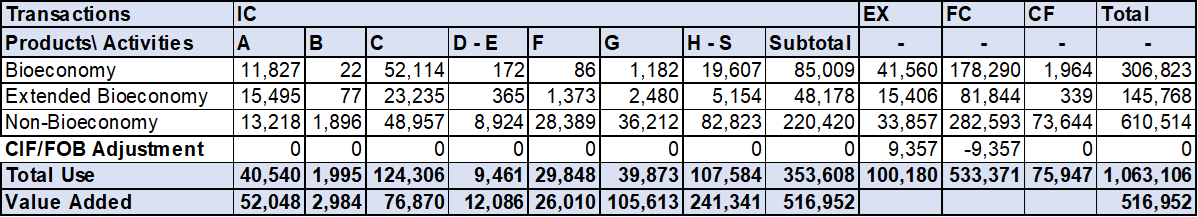
\includegraphics{images/clipboard-4242498611.png}

}

\end{table}%

Transactions: IC. Intermediate Consumption; EX. Exports; FC. Final
Consumption; CF. Capital Formation. Groups of Activities: A.
Agriculture; B. Mining; C. Manufacturing; D-E Other Utilities \& Water;
F. Construction; G. Wholesale and Retail Trade; H-S. Other services.

The remainder that results from subtracting intermediate consumption at
purchaser's prices from production at producer's prices (which is
technically known as gross output) is equal to gross Value Added (see
Table~\ref{tbl-gtm19-use}). This is calculated for each economic
activity (or column). Gross Value Added is similar to the profit that
results from subtracting the cost of inputs (excluding labor) from total
sales in a company, but at the level of the entire economy. The sum of
the value added by all economic activities, plus total taxes on
products, minus subsidies on those products, results in the Gross
Domestic Product (GDP). In this case, 926.4 billion -- 369.7 billion +
36.1 billion quetzales results a GDP of 592.8 billion GTQ for 2019.

If we were to abide by the \emph{a priori} selection of Bioeconomic
sectors, these would account for 17.0\% of gross Value Added---i.e.~the
Bioeconomy's GDP---, 4.6\% for extended bioeconomic activities, and
78.4\% for non-bioeconomic activities. However, we have explained the
limitations that come with that approach. That's why we suggest that
biological resources, as the natural resource basis of production across
\emph{all} economic activities (not just some), can be seen as a
spectrum. Each activity can make greater or lesser use of biological
inputs. In other words, each activity may have a higher or lower share
of bioeconomic products in its intermediate consumption structure and
can also produce a mix of products with a higher or lower proportion of
bioeconomic content. For this reason, estimating a bioeconomic
contribution of 17.0\% of Value Added, or 94.8 billion GTQ, overlooks in
some way the 997.5 million GTQ in bioeconomic products and the 42.2
billion GTQ in extended bioeconomic products produced by non-bioeconomic
activities. It would be more accurate to say that the value added across
all sectors was based on 24.0\% bioeconomic inputs (as explained earlier
in the intermediate consumption analysis), which is a calculation that
can be done individually for each sector (for example, agriculture,
manufacturing, and trade), without relying on the three bioeconomic
classification categories in the columns and instead focusing on the
bioeconomic content of products in the rows. The conclusion is that all
economic activities can be more or less bioeconomic, whether from the
perspective of production or intermediate consumption.

Table~\ref{tbl-gtm19-use} also shows exports, which total 95.3 billion
GTQ (excluding the CIF/FOB adjustments row), with 46.4\% corresponding
to bioeconomic products, 16.7\% to extended bioeconomic products, and
36.9\% to non-bioeconomic products. This is reasonable for a country
where a significant portion of exports consists of agricultural
products. Finally, of the 578.3 billion quetzales corresponding to final
consumption (excluding CIF/FOB adjustments), 32.8\% corresponds to
bioeconomic products, 15.0\% to extended bioeconomic products, and
52.2\% to non-bioeconomic products.

\subsubsection{Disaggregation by Economic
Activity}\label{disaggregation-by-economic-activity}

For a more detailed view of the Bioeconomy, we turn our attention to the
example of Costa Rica. Bioeconomic SUTs include detailed information on
hundreds of products and economic activities. Policy analysis can
benefit from this level of disaggregation when conducting sectoral
analyses. Table~\ref{tbl-cr18-pharma} shows an example of such a
detailed view of the Bioeconomy for the case of the pharmaceutical
sector of Costa Rica. Table~\ref{tbl-cr18-pharma} shows that 34.6\% of
the inputs of this economic activity by value depend on 24 bioeconomic
products. An additional 17.5\% of its Intermediate Consumption is
catalogued as belonging to the extended bioeconomy, while 47.9 percent
is accounted for by non-bioeconomic products.

\begin{longtable}[]{@{}
  >{\raggedright\arraybackslash}p{(\columnwidth - 4\tabcolsep) * \real{0.5068}}
  >{\raggedleft\arraybackslash}p{(\columnwidth - 4\tabcolsep) * \real{0.2466}}
  >{\raggedleft\arraybackslash}p{(\columnwidth - 4\tabcolsep) * \real{0.2466}}@{}}
\caption{Costa Rica: Pharmaceutical Sector Bioeconomy Intermediate
Consumption\\
(Million CRC at current prices and percent,
2018)}\label{tbl-cr18-pharma}\tabularnewline
\toprule\noalign{}
\begin{minipage}[b]{\linewidth}\raggedright
\textbf{Products}
\end{minipage} & \begin{minipage}[b]{\linewidth}\raggedleft
\textbf{Value (CRC)}
\end{minipage} & \begin{minipage}[b]{\linewidth}\raggedleft
\textbf{Percent}
\end{minipage} \\
\midrule\noalign{}
\endfirsthead
\toprule\noalign{}
\begin{minipage}[b]{\linewidth}\raggedright
\textbf{Products}
\end{minipage} & \begin{minipage}[b]{\linewidth}\raggedleft
\textbf{Value (CRC)}
\end{minipage} & \begin{minipage}[b]{\linewidth}\raggedleft
\textbf{Percent}
\end{minipage} \\
\midrule\noalign{}
\endhead
\bottomrule\noalign{}
\endlastfoot
\textbf{Bioeconomy (subtotal)} & \textbf{30,307.1} & \textbf{34.61\%} \\
Pharmaceutical and medicinal products & 18,845.6 & 21.52\% \\
Other food products n.e.c. & 4,011.2 & 4.58\% \\
Prepared animal feed & 2,624.9 & 3.00\% \\
Paper and paper products & 1,124.2 & 1.28\% \\
Garments & 1,063.4 & 1.21\% \\
Food and beverage supply services & 996.0 & 1.14\% \\
Other milling products n.e.c., starches, and starch derivatives & 582.7
& 0.67\% \\
Soaps, detergents, perfumes, and toiletries & 253.7 & 0.29\% \\
Products from non-perennial and perennial plants & 198.5 & 0.23\% \\
Wood and cork, wood and cork products, except furniture; articles of
straw and plaiting materials & 174.1 & 0.20\% \\
Support services for agriculture, livestock, and post-harvest activities
& 133.8 & 0.15\% \\
Vegetable and animal fats and oils & 107.9 & 0.12\% \\
Leather and related products, except footwear & 64.1 & 0.07\% \\
Rubber products & 41.3 & 0.05\% \\
Cane sugar, molasses, syrups, and other sugars & 39.3 & 0.04\% \\
Ground coffee, soluble coffee, extracts, and concentrates & 31.5 &
0.04\% \\
Wastewater evacuation services & 9.5 & 0.01\% \\
Cocoa, chocolates, and confectionery products & 1.8 & 0.002\% \\
Wheat flour & 1.5 & 0.002\% \\
Products from forestry, wood extraction, and hunting & 1.0 & 0.001\% \\
Eggs & 0.7 & 0.001\% \\
Dairy products & 0.1 & 0.0001\% \\
Other fruits, nuts, and other oil-bearing fruits & 0.1 & 0.0001\% \\
\textbf{Extended Bioeconomy (subtotal)} & \textbf{15,298.4} &
\textbf{17.47\%} \\
Basic chemicals and fertilizers, nitrogen compounds, pesticides, and
other agrochemical products & 14,232.3 & 16.25\% \\
Other manufactured products & 555.7 & 0.63\% \\
Textile products, except garments & 237.9 & 0.27\% \\
Waste collection, treatment, and disposal services; material recovery &
107.4 & 0.12\% \\
Scientific research and development services & 65.6 & 0.07\% \\
Building cleaning and landscape care and maintenance & 46.7 & 0.05\% \\
Drinking water & 45.2 & 0.05\% \\
Waste and scraps & 6.8 & 0.01\% \\
Footwear & 0.7 & 0.001\% \\
\textbf{Non-Bioeconomy (subtotal)} & \textbf{41,960.0} &
\textbf{47.92\%} \\
Remaining 68 Non-Bioeconomy products. & 41,960.0 & 47.92\% \\
\textbf{Total Use} & \textbf{87,565.5} & \textbf{100.00\%} \\
\end{longtable}

Source: Own elaboration based on Costa Rica's SUTs (BCCR, 2021a).

BSAs can be used to perform this type of exploration for sectors of
interest in the context of an economic policy. For example, we can see
that biological resources are very important in the case of the
processed foods industry, both for \emph{Meat Products}
(Figure~\ref{fig-meat-products}) and \emph{Milk and Dairy}
(Figure~\ref{fig-dairy}) where Bioeconomy products make up 81 and 76
percent of their intermediate consumption, respectively. In contrast,
Bioeconomic products account for only 4 percent of the value of
intermediate consumption in the \emph{Residential Construction} sector
(Figure~\ref{fig-construction}). Given a policy that provides incentives
for the use of innovative biological materials in construction, for
example, policy-makers could focus on monitoring the increase or
decrease of this share over time.

\begin{figure}

\begin{minipage}{0.33\linewidth}

\centering{

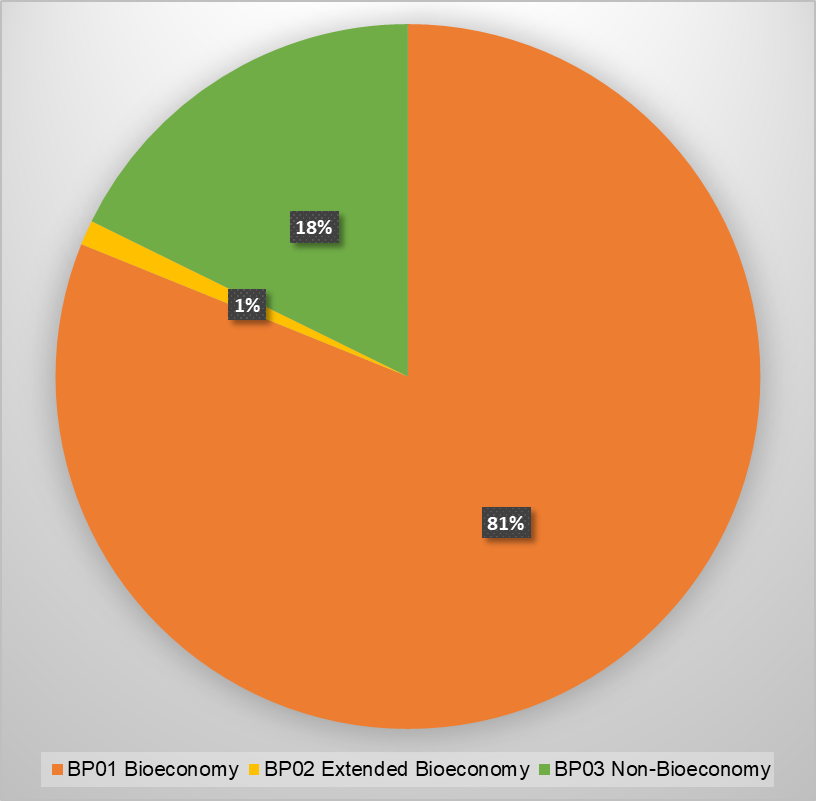
\includegraphics{images/clipboard-2928692590.png}

}

\subcaption{\label{fig-meat-products}Meat products}

\end{minipage}%
%
\begin{minipage}{0.33\linewidth}

\centering{

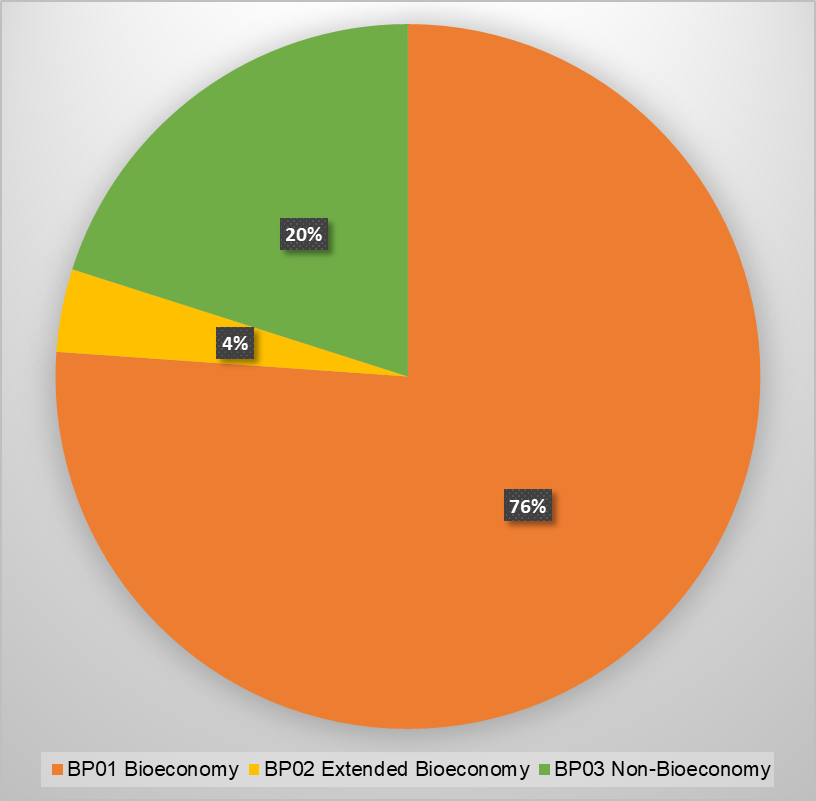
\includegraphics{images/clipboard-2666308793.png}

}

\subcaption{\label{fig-dairy}Milk and Dairy}

\end{minipage}%
%
\begin{minipage}{0.33\linewidth}

\centering{

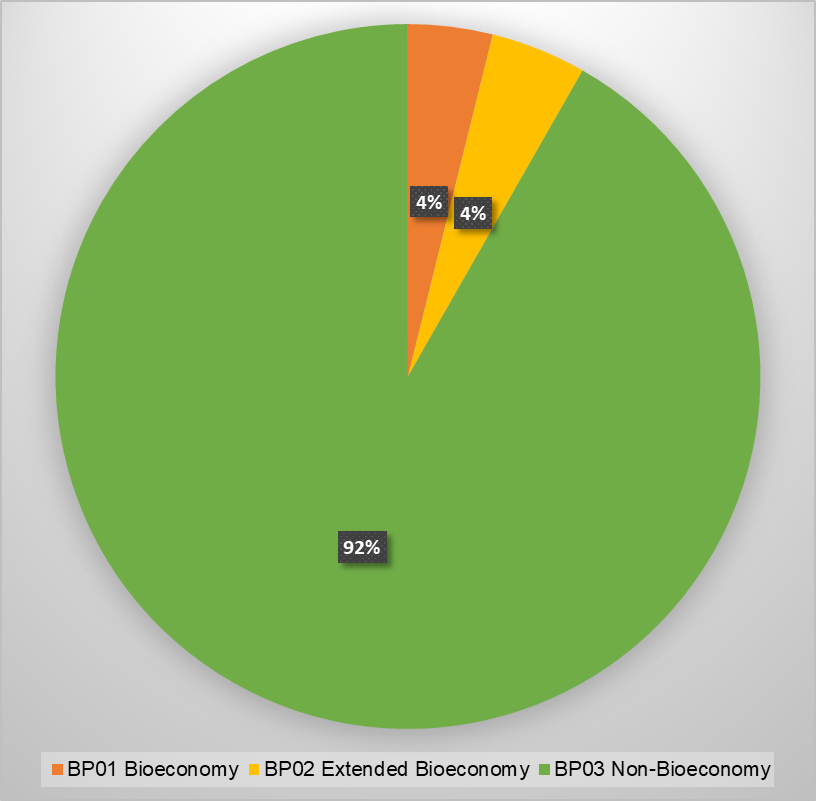
\includegraphics{images/clipboard-1429514424.png}

}

\subcaption{\label{fig-construction}Construction}

\end{minipage}%

\caption{\label{fig-cri-sectoral}Bioeconomy, Extended Bioeconomy, and
Non-Bioeconomy inputs for selected economic activities~ (Costa Rica,
percent, 2018)}

\end{figure}%

\subsubsection{Comparative analysis for 13 economies of Latin America
and The
Caribbean}\label{comparative-analysis-for-13-economies-of-latin-america-and-the-caribbean}

Following the same analytical approach used in Table~\ref{tbl-gtm19-sup}
for the case of Guatemala, the panels in Figure~\ref{fig-latam-output}
provide a comparative analysis of the percentage contribution of the
Bioeconomy to several SNA transactions for Argentina, Brazil, Chile,
Colombia, Costa Rica, El Salvador, the Dominican Republic, Ecuador,
Guatemala, Honduras, Nicaragua, Panama, and Peru. While the analysis for
Guatemala was developed for the year 2019, the focus of this section is
the year 2018, since it is the most recent year available for the
majority of the countries, with the exception of the Dominican Republic
and Panama, where 2016 and 2017 data, respectively, were used.

Figure~\ref{fig-latam-imports} shows that, on average, 17.5\% of gross
output in the analyzed countries corresponds to bioeconomic products,
10.6\% to extended bioeconomic products, and 71.9\% to non-bioeconomic
products. Nicaragua has the highest proportion of bioeconomic products,
with about a third of its output (29.1\%) falling into this category.
This highlights a broader agricultural base in their economy. Panama, on
the other hand, ranks the lowest, with 11.5\% of bioeconomic products in
its national production structure. However, its proportion of extended
bioeconomic products reaches 9.9\%, and when combined, these two
categories account for one-fifth of its production based on biological
resources.

The importance of the bioeconomy in imports is illustrated in
Figure~\ref{fig-latam-imports}, which shows that Costa Rica has the
highest level of bioeconomic imports, representing 27.1\% of its total
imports. In contrast, Argentina and Brazil have the lowest levels, with
6.0\% of their imports being bioeconomic products. It's worth examining
the combined participation of bioeconomic and extended bioeconomic
products in some cases, though caution is advised when interpreting
extended bioeconomic products, as it is not always possible to determine
the purely biological share due to the aggregation level of product
classification in national accounts. For example, Honduras sits in the
middle of the chart with 12.2\% of its imports being bioeconomic, but
40.1\% of its imports fall under extended bioeconomic products.
Combined, half of its imports are based on biological resources
(52.3\%). On average, across all the countries analyzed, bioeconomic
products represent 12.5\% of imports, extended bioeconomic products
19.5\%, and non-bioeconomic products 68.0\%.

Costa Rica is the country that derives the highest fiscal revenue from
bioeconomic products, which account for 32.7\% of taxes minus subsidies
on products, as shown in Figure~\ref{fig-latam-tax}. At the other end of
the spectrum, bioeconomic products in Panama are responsible for 13.9\%
of that revenue. It's also worth comparing the combined total for
bioeconomic and extended bioeconomic products. In that case, Panama
reaches 37.4\%, while Costa Rica, which has only 4.3\% attributable to
extended bioeconomic products, totals 37.0\%. On average, across the
analyzed countries, 24.5\% of taxes come from bioeconomic products,
16.0\% from extended bioeconomic products, and 59.5\% from
non-bioeconomic products.

\begin{figure}

\begin{minipage}{\linewidth}

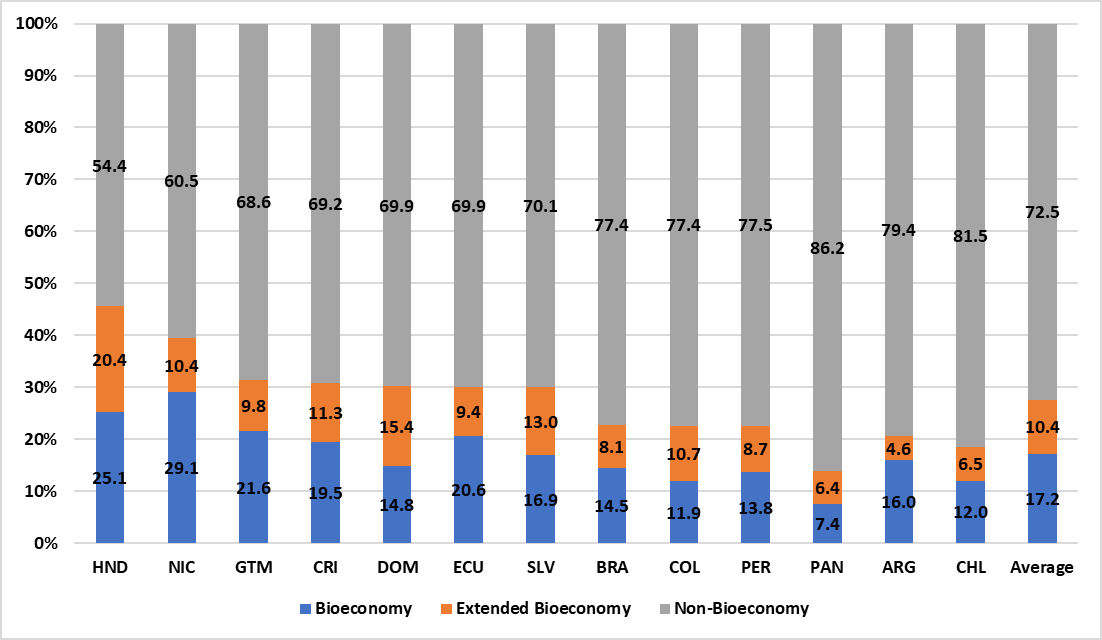
\includegraphics{images/clipboard-641492741.png}

\subcaption{\label{}Gross Output}
\end{minipage}%
\newline
\begin{minipage}{\linewidth}

\centering{

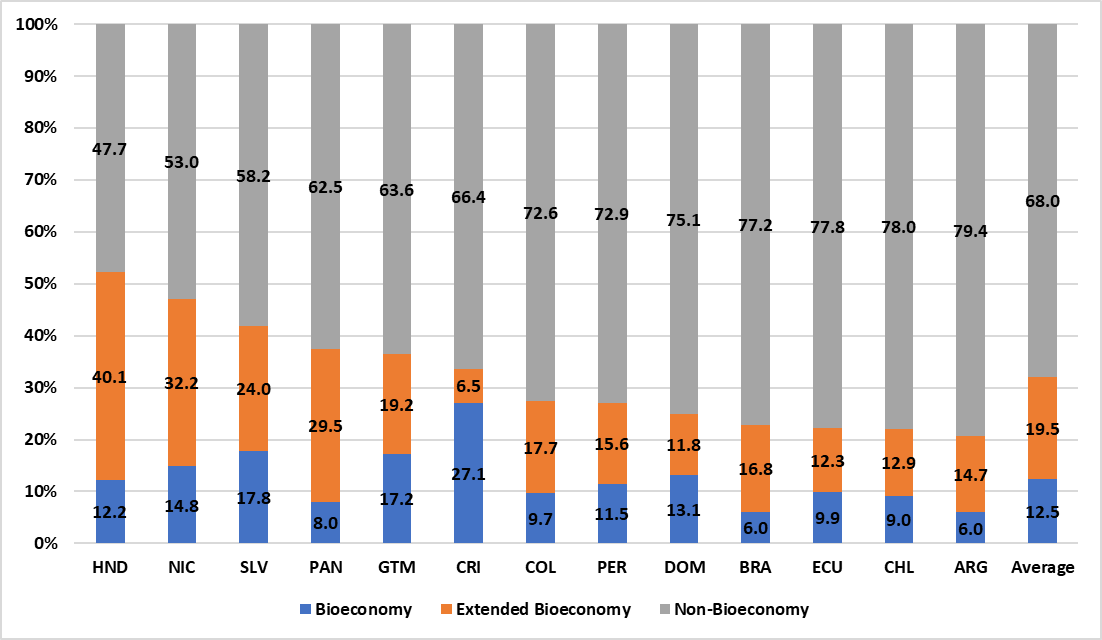
\includegraphics{images/clipboard-4077757569.png}

}

\subcaption{\label{fig-latam-imports}Imports}

\end{minipage}%
\newline
\begin{minipage}{\linewidth}

\centering{

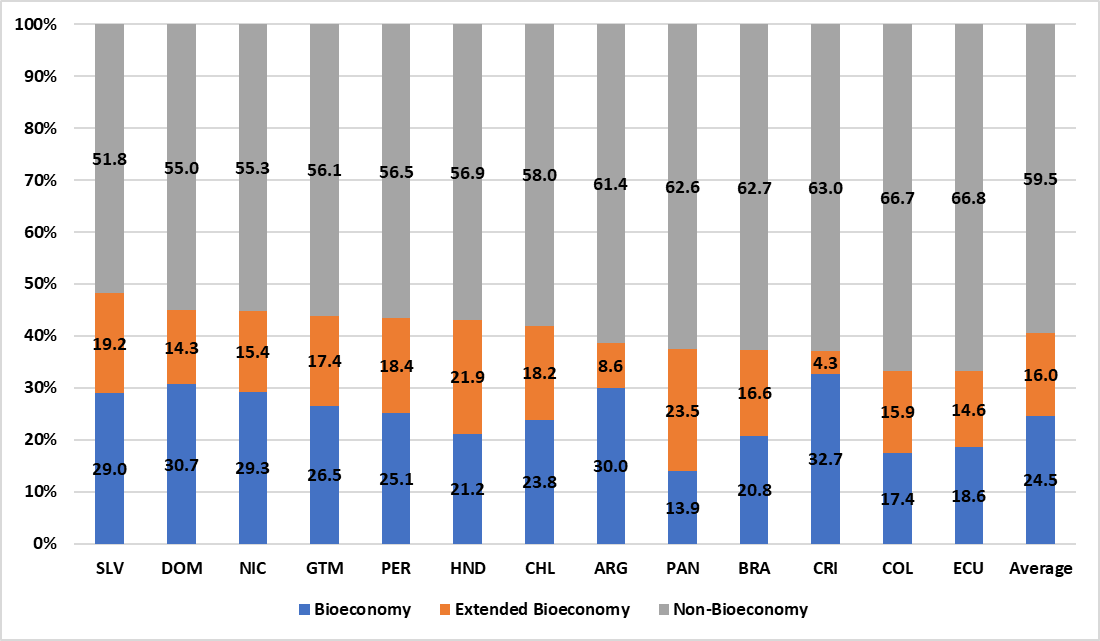
\includegraphics{images/clipboard-1372132090.png}

}

\subcaption{\label{fig-latam-tax}Taxes less subsidies}

\end{minipage}%

\caption{\label{fig-latam-output}Supply Table Transactions (13 Latin
American Economies, percent, 2018)}

\end{figure}%

At this point, it's helpful to revisit the concept of the implicit tax
rate on bioeconomic products, as explained earlier for the case of
Guatemala. Figure~\ref{fig-latam-implicit-tax} shows these rates, along
with the implicit rates for extended bioeconomic products and
non-bioeconomic products for the 13 countries analyzed, as well as the
group average. These rates are calculated by dividing total tax revenue
for a specific type of product by the total production of that same
product type. As explained earlier, it's important to understand that
these rates are not the result of a deliberate fiscal policy regarding
the bioeconomy but simply the current net outcome across the three
product types from various tax instruments implemented at different
times for diverse purposes. Argentina has the highest tax rate on
bioeconomic products, with an implicit rate of 17.8\%, which is 2.4
times higher than the 7.3\% rate on non-bioeconomic products. This
disparity, which imposes significantly higher taxes on bioeconomic
products compared to non-bioeconomic ones, is observed in at least 11 of
the 13 countries analyzed (Argentina, Brazil, Chile, El Salvador, the
Dominican Republic, Peru, Colombia, Costa Rica, Nicaragua, Guatemala,
and Panama), as well as in the overall average, where bioeconomic
products have an implicit tax rate of 8.2\%, extended bioeconomic
products 9.1\%, and non-bioeconomic products 4.5\%. The case of Honduras
is interesting, where the trend is reversed, and bioeconomic products
have a lower implicit rate (4.3\%) than non-bioeconomic products
(5.3\%). A similar situation occurs in Ecuador (3.8\% and 4.1\%,
respectively).

\begin{figure}

\centering{

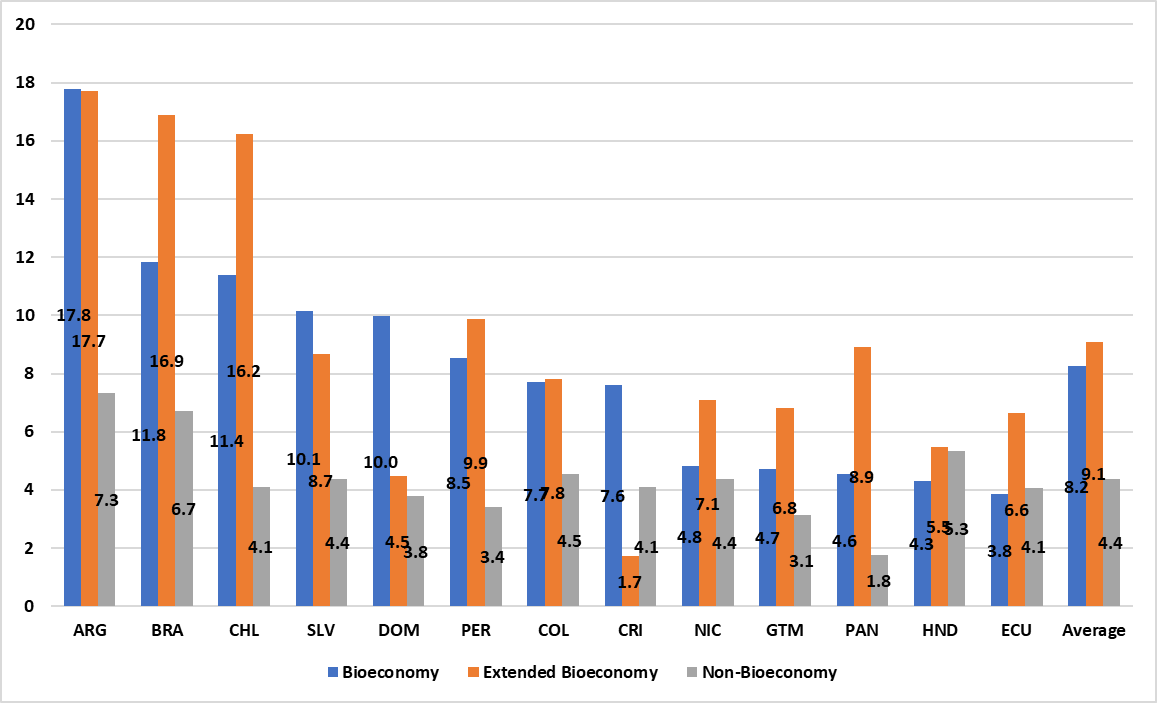
\includegraphics{images/clipboard-1492103812.png}

}

\caption{\label{fig-latam-implicit-tax}Implicit Tax Rate (13 Latin
American Economies, percent, 2018)}

\end{figure}%

Figure~\ref{fig-latam-use} compares three use-side transactions across
the analyzed countries. First, in
Figure~\ref{fig-latam-intermediate-consumption}, bioeconomic products
represent, on average, 18.6\% of intermediate consumption, extended
bioeconomic products 13.3\%, and non-bioeconomic products 68.0\%, across
the 13 countries analyzed. Nicaragua is the country whose production
relies most heavily on a bioeconomic base, with its intermediate
consumption of these products reaching 26.5\%, followed by Guatemala
(24.0\%) and Ecuador (23.0\%) at the top of the chart. In contrast,
Colombia (12.2\%), Chile (12.2\%), and Panama (12.0\%) occupy the last
three positions. Once again, it's worth highlighting the case of
Honduras, where the share of extended bioeconomic products (29.3\%),
combined with bioeconomic products (29.3\%), means that more than half
of the country's intermediate consumption (51.9\%) is linked to
biological resources.

In the case of exports, shown in Figure~\ref{fig-latam-exports}, Ecuador
(47.0\%), Argentina (45.8\%), and Nicaragua (44.0\%) are the three
countries with the highest percentage of exports consisting of
bioeconomic products, while Colombia (14.2\%), the Dominican Republic
(13.1\%), and Panama (4.0\%) have the lowest values. This is closely
tied to the importance of agricultural products in the export structure
of each country.

Finally, the final consumption shown in
Figure~\ref{fig-latam-final-consumption}, which includes household
consumption, government consumption, and nonprofit institutions'
consumption, plays a key role as a driver of the economy, directly and
indirectly influencing production and import decisions in economic
activities. In this case, Costa Rica has the highest proportion of its
consumption attributed to bioeconomic products (36.4\%), followed by
Guatemala (31.7\%) and Honduras (31.7\%) at the top. Panama and Brazil
(both at 18.9\%), Colombia (18.5\%), and Chile (18.2\%) occupy the
lowest positions.

\begin{figure}

\begin{minipage}{\linewidth}

\centering{

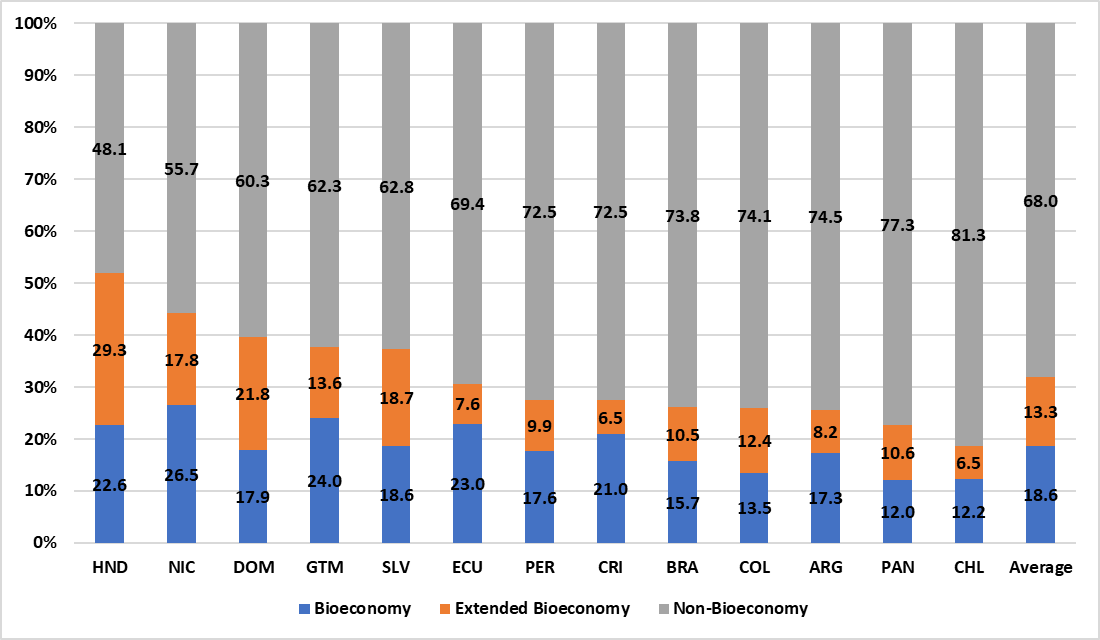
\includegraphics{images/clipboard-2112192972.png}

}

\subcaption{\label{fig-latam-intermediate-consumption}Intermediate
Consumption}

\end{minipage}%
\newline
\begin{minipage}{\linewidth}

\centering{

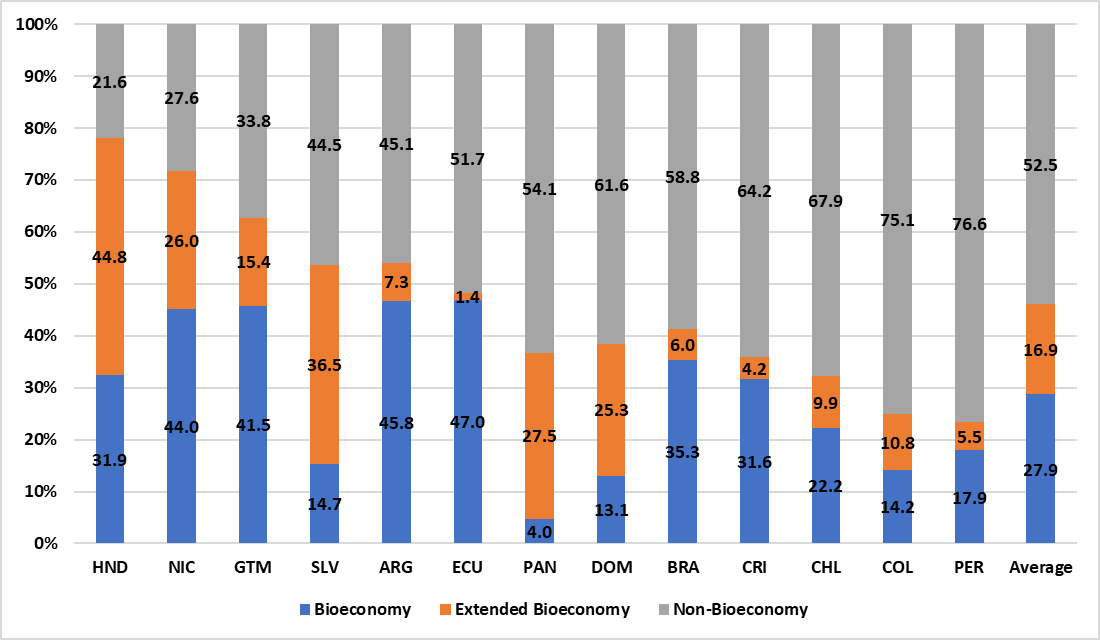
\includegraphics{images/clipboard-995186152.png}

}

\subcaption{\label{fig-latam-exports}Exports}

\end{minipage}%
\newline
\begin{minipage}{\linewidth}

\centering{

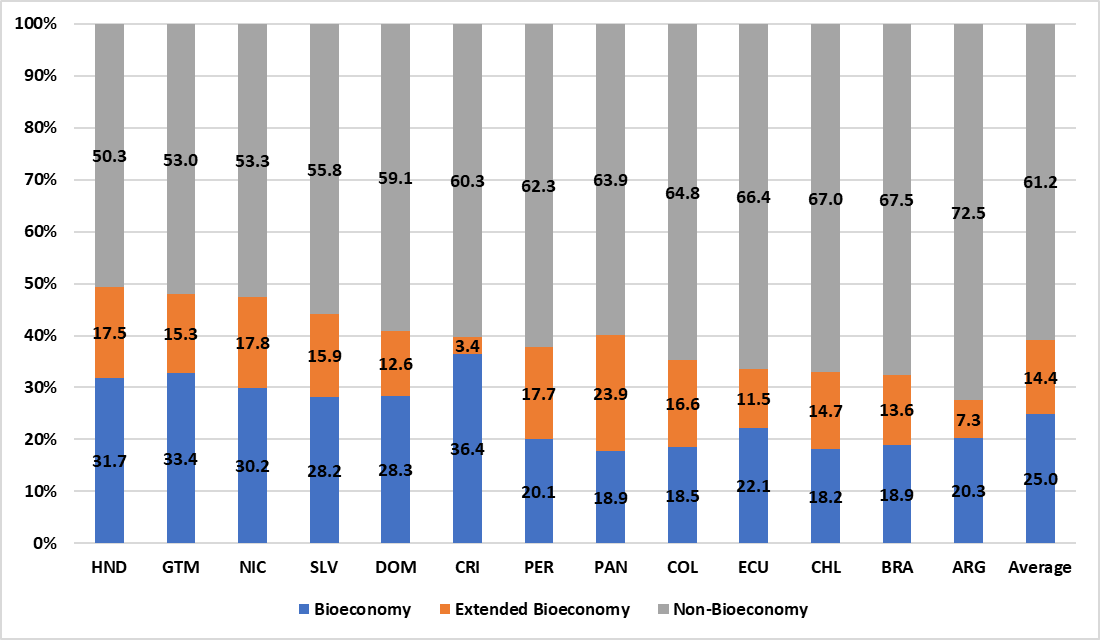
\includegraphics{images/clipboard-1453266958.png}

}

\subcaption{\label{fig-latam-final-consumption}Final Consumption}

\end{minipage}%

\caption{\label{fig-latam-use}Use Table Transactions (13 Latin American
Economies, percent, 2018)}

\end{figure}%

If we consider that intermediate consumption is the input base for
producing all the goods and services in the economy, the percentages
shown for this transaction suggest that between 12.0\% and 26.5\% of the
value added in the region's countries is based on biological resources,
with an average of 18.6\%. This analysis can also be applied at a
sectoral level, identifying the shares of intermediate consumption that
correspond to the bioeconomy for each major sector group, as shown in
Figure~\ref{fig-latam-avg-sector-biocontent}. This reveals that, for the
years analyzed and on average for the countries, 44.3\% of the value
added in agriculture is generated based on the intermediate consumption
of bioeconomic products. Following this, 34.8\% of the value added in
manufacturing industries is based on bioeconomic resources. Other
services ranks third, with 11.2\% of its intermediate consumption
corresponding to bioeconomic products, supporting its value-added
generation. In contrast, mining, utilities, construction, and trade have
between 0.6\% and 2.0\% of their intermediate consumption made up of
bioeconomic products, suggesting that these products play a less direct
role in generating value added in these sectors.

\begin{figure}

\centering{

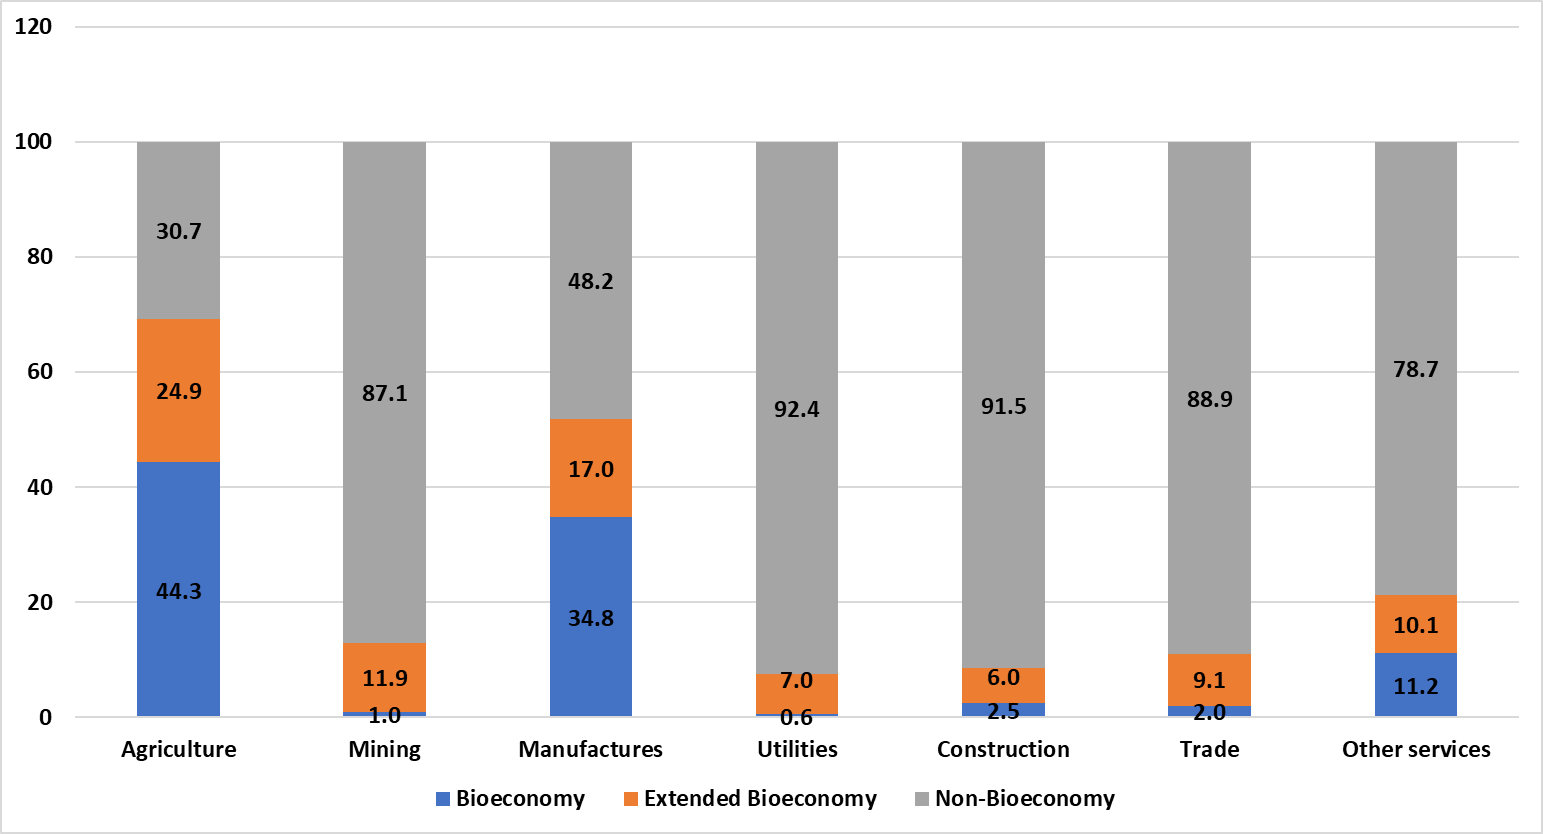
\includegraphics{images/clipboard-3829818055.png}

}

\caption{\label{fig-latam-avg-sector-biocontent}Average bioeconomic
content value in intermediate consumption by aggregated groups of
economic activity (13 Latin American Economies, percent, 2018)}

\end{figure}%

Finally, we explore the contribution of the bioeconomy to GDP. To
provide some context, the sum of the value added by economic activities,
plus taxes net of subsidies, makes up the Gross Domestic Product (GDP).
Value added is a measure calculated at the level of economic activities,
not at the product level. For this reason, it is common for studies
determining the contribution of the bioeconomy to the economy to
classify economic activities as ``bioeconomic'' a priori and then simply
add up their value added to determine their contribution to GDP. In
fact, we have also replicated this approach in our own work. However, we
have realized that, given that in the national accounts system, products
can be produced by more than one activity and each activity can produce
more than one product, choosing bioeconomic sectors a priori leads to
excluding the contribution of products that we have identified as
bioeconomic but are not produced or consumed by activities classified as
bioeconomic. In most cases, this leads to an underestimation of the
contribution of the bioeconomy.

As we explained earlier, we suggest it is more useful to consider the
bioeconomic status of activities as a spectrum, making them more or less
dependent on bioeconomic products depending on the amount of bioeconomic
inputs present in their intermediate consumption.
Figure~\ref{fig-latam-value-added-methods} presents a comparative
analysis of the percentage of the economy that can be attributed to the
bioeconomy, depending on whether the value added is adjusted as a
percentage of intermediate consumption, weighted by each sector's
contribution to the total (via Intermediate Consumption in the table),
or if the entire value added of sectors considered a priori to be
bioeconomic or extended bioeconomic is taken (via sector catalog in the
table). What is revealing is that in most cases, except for Chile,
Ecuador, and Nicaragua, the estimation obtained by assigning sectors a
priori underestimates the contribution of the bioeconomy to GDP by
several percentage points.

\begin{figure}

\centering{

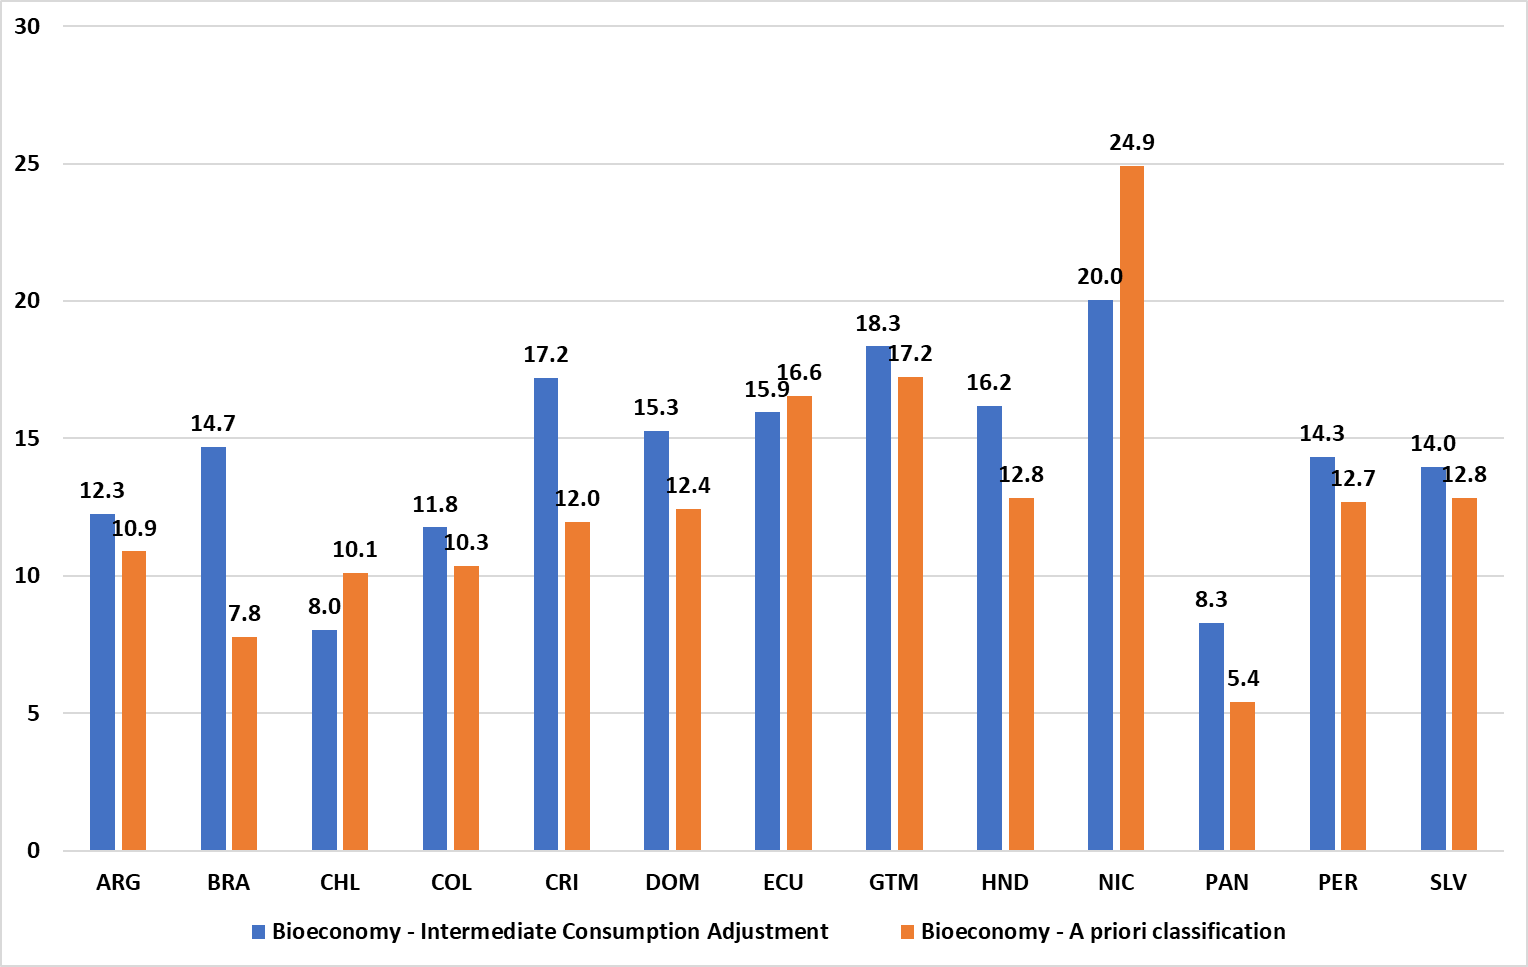
\includegraphics{images/clipboard-535496738.png}

}

\caption{\label{fig-latam-value-added-methods}Comparison of Bioeconomy
contribution to Value Added by method of adjustment (13 Latin American
Economies, percent, 2018)}

\end{figure}%

\subsection{Closing arguments}\label{closing-arguments}

We have shown the results of applying a standardized methodology for
constructing Bioeconomy Satellite Accounts to the Supply and Use Tables
of the National Accounts Systems of 13 countries from Latin America and
The Caribbean Argentina, Brazil, Chile, Colombia, Costa Rica, El
Salvador, the Dominican Republic, Ecuador, Guatemala, Honduras,
Nicaragua, Panama, and Peru.

Among the key findings of this exercise, we find that, in the region,
bioeconomic products account for 17.5\% of production, 12.5\% of
imports, 24.5\% of product-related taxes, 8.6\% of intermediate
consumption, 27.9\% of exports, and 25\% of household final consumption
on average.

A significant share of fiscal revenue from product taxes comes from
bioeconomic products (ranging from 13.9\% to 32.7\% for the countries
analyzed). By dividing tax revenue by product type and the gross
production value of those goods, it is possible to estimate the implicit
tax rate. It's important to note that for most countries, this implicit
rate is considerably higher for bioeconomic products than for
non-bioeconomic ones. This disparity is not intentional but rather the
combined result of different fiscal policy instruments created at
various times for diverse purposes. In the context of developing public
policies related to the Bioeconomy, it is crucial to explore this issue
further in order to create incentive mechanisms that foster bioeconomic
development while balancing public finance objectives.

One limitation of the National Accounts data for studying the bioeconomy
is related to the difficulty in quantifying bioeconomic gross capital
formation through economic surveys and business financial statements. A
significant portion of innovation in the Bioeconomy is related to
intellectual property, and companies in the region still face challenges
in tracking their intellectual assets and accurately accounting for
them. Another challenge in quantifying bioeconomic Gross Capital
Formation arises from the fact that some infrastructure projects may not
be easily identified as bioeconomic, such as the construction of
bioprocessing plants to reuse biological waste. These would typically
appear under construction services and would be excluded by the
methodology during the classification process. This indicates that there
is still work to be done in developing national accounting standards to
address these limitations.

\subsection{Acknowledgments}\label{acknowledgments}

The methodology described here was originally developed for Costa Rica
through a collaboration between the Central Bank of Costa Rica (BCCR)
and the United Nations Economic Commission for Latin America and the
Caribbean (ECLAC), at the request of Costa Rica's National Council of
Environmental Accounts. Financing was provided by the German Cooperation
(\emph{Deutsche Gesellschaft für Internationale
Zusammenarbeit}---GIZ---GmbH) for the lead author's time. Technical
support and oversight, as well as data access, were kindly provided by
the Central Bank of Costa Rica and ECLAC who assigned time from the
remaining authors to this task. We are particularly grateful for the
Costa Rican Council of Environmental and Economic Accounts
representative Cynthia Córdoba's political, institutional, and
administrative arrangements to facilitate this work. We also appreciate
the insightful comments offered by the anonymous peer reviewers. The
views expressed here remain the authors' responsibility and do not
reflect official positions of any of the institutions involved.

\phantomsection\label{refs}
\begin{CSLReferences}{1}{0}
\bibitem[\citeproctext]{ref-bccr_cuadro_2021}
BCCR. (2021a). \emph{Cuadro de oferta y utilización 2018}. San José de
Costa Rica: Banco Central de Costa Rica. Retrieved from Banco Central de
Costa Rica website:
\url{https://www.bccr.fi.cr/indicadores-economicos/cuentas-nacionales-periodo-de-referencia-2017}

\bibitem[\citeproctext]{ref-bccr_cuentas_2021}
BCCR. (2021b). \emph{Cuentas {Ambientales} de {Costa} {Rica}: {Cuadro}
de {Oferta} y {Utilización} de {Flujos} {Físicos} de {Energía} 2018}.
San José de Costa Rica: Banco Central de Costa Rica.

\bibitem[\citeproctext]{ref-bowers2019}
Bowers, J., \& Testa, P. F. (2019). Better Government, Better Science:
The Promise of and Challenges Facing the Evidence-Informed Policy
Movement. \emph{Annual Review of Political Science}, \emph{22}(Volume
22, 2019), 521--542.
\url{https://doi.org/10.1146/annurev-polisci-050517-124041}

\bibitem[\citeproctext]{ref-eclac2021}
ECLAC. (2021). \emph{{Repository} of {Supply} and {Use Tables} and
{Input-Output Matrices} from {Latin America} and {The Caribbean}}.
Retrieved from
\url{https://statistics.cepal.org/repository/cou-mip/index.html?lang=es}

\bibitem[\citeproctext]{ref-europeancommission2013}
European Commission, Economic Cooperation, O. for, Development, United
Nations, \& World Bank. (2013). \emph{{System} of
{Environmental}-{Economic} {Accounting} {2012}}. New York.

\bibitem[\citeproctext]{ref-europeancommission2009}
European Commission, International Monetary Fund, Economic Co-operation,
O. for, Development, United Nations, \& World Bank. (2009).
\emph{{System} of {National} {Accounts} {2008}}. Retrieved from
\url{https://unstats.un.org/unsd/nationalaccount/sna2008.asp}

\bibitem[\citeproctext]{ref-germanbioeconomycouncil2018}
German Bioeconomy Council. (2018). \emph{{Global} {Bioeconomy} {Summit}:
{Conference} {Report}. {Innovation} in the {Global} {Bioeconomy} for
{Sustainable} and {Inclusive} {Transformation} and {Wellbeing}}. Berlin.

\bibitem[\citeproctext]{ref-gobiernodecostarica2020}
Gobierno de Costa Rica. (2020). \emph{Estrategia {Nacional} de
{Bioeconomía Costa Rica} 2020 - 2030: {Hacia} una economía con
descarbonización fósil, competitividad, sostenibilidad e inclusión}. San
José de Costa Rica. Retrieved from
\url{https://www.micit.go.cr/sites/default/files/estrategia_nacional_bioeconomia_cr_corregido.pdf}

\bibitem[\citeproctext]{ref-unitednations2008}
United Nations. (2008). \emph{{International} {Standard} {Industrial}
{Classification} of {All} {Economic} {Activities}: {Revision} 4}. New
York. Retrieved from
\url{https://unstats.un.org/unsd/classifications/Econ/isic}

\bibitem[\citeproctext]{ref-unitednations2015}
United Nations. (2015). \emph{{Central} {Product} {Classification} (CPC)
{Version} 2.1}. New York. Retrieved from
\url{https://unstats.un.org/unsd/classifications/Econ/cpc}

\bibitem[\citeproctext]{ref-vargas2022}
Vargas, R., Alvarado, I., Rodríguez, M., Rodríguez, A., \& Wander, P.
(2022). \emph{Cuenta satélite de bioeconomía para Costa Rica: Propuesta
metodológica y aplicación práctica}. Santiago de Chile: Comisión
Económica para América Latina y el Caribe. Retrieved from
\url{https://www.cepal.org/es/publicaciones/48641-cuenta-satelite-bioeconomia-costa-rica-propuesta-metodologica-aplicacion}

\end{CSLReferences}



\end{document}
